\chapter[Metodologia]{Metodologia}
%rever esse trecho
Esse capítulo aborda diversos tipos de metodologias e procedimentos de pesquisa, bem como caracteriza a metodologia utilizada durante o desenvolvimento da pesquisa deste trabalho. O capítulo está organizado em seções. Na seção 5.1, é explanado sobre as classificações de pesquisa quanto ao objetivo e aos procedimentos técnicos. Em seguida, na seção 5.2, é apresentada a metodologia aplicada tanto para pesquisa quanto para o desenvolvimento do software, bem como relatado o fluxo de atividades e a execução dessas atividades conforme o cronograma.

 \section{Classificações de Metodologias de Pesquisa}
  
Pesquisar pode ser entendido como uma realização concreta de uma investigação planejada, desenvolvida e redigida de acordo com as normas da metodologia consagradas pela ciência, ou, de forma mais simples, como uma atividade para solucionar problemas \cite{kauark2010} \cite{ruiz1996}. 

 \par
  \indent Utilizando objetivo geral como critério de classificação, pode-se categorizar as pesquisas em três grupos: exploratória, descritiva e explicativa. A pesquisa exploratória busca obter maior conhecimento sobre um assunto específico ainda pouco conhecido tornando-o mais explícito e orientando à formulação de hipóteses \cite{gil2002}. Geralmente, é realizada em forma de estudo de caso ou pesquisa bibliográfica \cite{rodrigues2007} e, para sua execução, costuma-se fazer uso de entrevistas com pessoas experientes no assunto, levantamento bibliográfico e análise de exemplos relacionados à temática \cite{gil2002}. 

 \par
  \indent A pesquisa descritiva propõe ao investigador descrever as características de uma população ou fenômeno, ou determinar a existência de relações de dependência entre variáveis \cite{gil2002}.  Em geral, é realizada com auxílio de coleta de dados por meio de questionários e observações sistemáticas \cite{tafner2007}. Para uma correta interpretação da pesquisa, é importante que o investigador observe, registre, analise e classifique os dados de forma que não haja interferências com os fatos observados \cite{rodrigues2007}. 

 \par
  \indent O terceiro grupo refere-se à pesquisa explicativa. Essa tem como objetivo explanar sobre os fatores que determinam ou contribuem com  a ocorrência de um fenômeno específico. Essa categoria de pesquisa visa compreender os motivos de um fenômeno, enquanto a exploratória e descritiva motivam-se a entender o fenômeno em si e detalhá-lo \cite{gil2002}. Comumente é realizada por meio de pesquisa  \textit{ex-post facto} e pesquisa experimental \cite{tafner2007}.

 \par
 \indent Embora a classificação quanto ao objetivo proporcione uma visão conceitual da pesquisa, existe a necessidade de obter uma visão a nível operativo \cite{gil2002}. Nesse sentido, pode-se categorizar pesquisas quanto ao procedimento técnico utilizado. Entre eles temos:
 
\begin{description}
\item[Pesquisa bibliográfica:] é realizada a partir do levantamento de referências teóricas sobre o tema. De forma geral, toda pesquisa inicia-se como uma pesquisa bibliográfica, mas há aquelas que dependem exclusivamente desse tipo de pesquisa. Em essência, a conclusão desse tipo de pesquisa é uma compilação das publicações referentes ao tema \cite{prodanov2013}.  

\item[Pesquisa documental:] semelhante à pesquisa bibliográfica, diferencia-se pela natureza das fontes. Tem como base documentos sem tratamento analítico, como tabelas, cartas fotos, pinturas, dentre outros \cite{gil2002}. 

\item[Pesquisa experimental:] seleciona grupos de assuntos coincidentes e submete-os a tratamentos diferentes. Com isso, ocorre uma verificação se há variáveis estranhas e é avaliado se as diferenças observadas nas respostas são estatisticamente significantes \cite{tafner2007}.

\item[Pesquisa \textit{ex-post facto}:] investiga possíveis relações de causa e efeito entre um determinado fato identificado pelo pesquisador e um fenômeno que ocorre posteriormente. A principal característica da pesquisa \textit{ex-post facto} é o fato dos dados serem coletados após a ocorrência dos eventos \cite{gil2002}.

\item[Levantamento (\textit{survey}):] utilizada em estudos exploratórios e descritivos, o levantamento pode ser de dois tipos: levantamento de uma amostra ou levantamento de uma população (também designado de censo). A coleta de dados realiza-se em ambos os casos por meio de questionários ou entrevistas. Em seguida, é realizada análise quantitativa dos dados e formuladas as possíveis conclusões \cite{prodanov2013}.

\item[Estudo de coorte:] diz respeito a um tipo de pesquisa em que seleciona um grupo de pessoas com uma característica comum. A partir de então, o grupo é acompanhado a fim de observar e analisar o que ocorre com elas num determinado tempo. Esse tipo de estudo pode ser categorizado em dois tipos: estudo retrospectivo e estudo prospectivo. O primeiro ocorre com a análise de dados históricos, enquanto o segundo refere-se à análise com dados atuais \cite{gil2002}.   

\item[Estudo de caso:] pode ser caracterizado de acordo com o estudo profundo de uma entidade bem definida como um programa, uma instituição, um sistema educativo, uma pessoa ou uma unidade social. Visa conhecer em profundidade o seu "como" e os seus "porquês", evidenciando suas unidade e identidade próprias \cite{prodanov2013}. 

\item[Estudo de campo:] similar ao levantamento, entretanto, o estudo de campo busca maior aprofundamento nas questões propostas. O pesquisador deve ser imerso na comunidade a ser estudada de forma a obter maior conhecimento sobre as regras que regem o grupo. Esse tipo de estudo pode ser realizado com observação direta das atividades, entrevistas e análise de documentos, fotografias e filmagens \cite{tafner2007}.

\item[Pesquisa-ação:] esse tipo de pesquisa é ciclíca e pressupõe uma participação planejada do pesquisador na situação problemática a ser investigada. Recorre a uma metodologia sistemática, no sentido de transformar as realidades observadas, a partir da sua compreensão, conhecimento e compromisso para a ação dos elementos envolvidos na pesquisa\cite{thiollent2009}. Embora seja considerada flexível para alguns autores, outros definem as fases planejar, agir, monitorar e avaliar como etapas da execução de uma pesquisa-ação \cite{ferreira2011}. 

\item[Pesquisa participante:] similar à pesquisa-ação, difere-se quanto ao planejamento da ação. Enquanto a pesquisa-ação requer um planejamento anterior à ação do pesquisador; a pesquisa participante não pressupõe essa atividade. Com a finalidade de adquirir maior compreensão do grupo, o investigador participa da comunidade e suas atividades. A finalidade do estudo e a identidade do investigador devem ser de ciência para todos os envolvidos \cite{tafner2007}.
\end{description}

 \section{Planejamento da Metodologia Aplicada}
  
Utilizando o estudo descrito anteriormente como base, foi definida a metodologia de pesquisa utilizada durante o desenvolvimento do trabalho de conclusão de curso, bem como uma adaptação de metodologia para o desenvolvimento do \textit{framework}, embasada em práticas do Scrum \cite{scrum2014} e do eXtreme Programming \cite{wells2009}.  
  
  \subsection{Metodologia de Pesquisa} \label{Metodologia de Pesquisa}
	O tipo de pesquisa adotado foi um misto de pesquisa exploratória, na medida em que se buscou criar maior familiaridade com a temática, e pesquisa experimental, onde objetivou-se averiguar o funcionamento do \textit{framework} com o uso de condições em ambiente controlado. 
  \par
  \indent Quanto ao procedimento técnico, a modalidade de pesquisa empregada foi pesquisa-ação. Dessa forma, fez-se uso de ciclos de coleta e análise de dados e desenvolvimento para alteração do objeto de estudo, conforme as análises do ciclo anterior.

 \subsection{Metodologia de Desenvolvimento do Software} \label{Metodologia de Desenvolvimento do Software}
  No que se refere ao desenvolvimento do software, utilizou-se uma adaptação do Scrum e eXtreme Programming. As \textit{Sprints} durante o desenvolvimento foram de quatorze dias e fez-se uso de algumas práticas como \textit{Planning Poker}, Padronização do Código, Programação em Pares \cite{wells2009}, estimativas relativas, \textit{timebox}, \textit{backlog}, definição de pronto e quadro de tarefas \cite{scrum2014}. 
 
 \subsection{Fluxo de Atividades Geral}
 	
 	Utilizando as metodologias definidas para a execução do trabalho de conclusão de curso 01 e 02, foi estabelecido um fluxo de atividades que possibilitou o alcance dos objetivos do projeto.
 	
 \par
 \indent Inicialmente, foram realizados estudos sobre a temática escolhida. Em seguida, foram determinados o escopo do projeto e a proposta inicial,, resumindo os objetivos, justificativa, cronograma preliminar, entre outros aspectos introdutórios que guiaram as atividades seguintes. O estudo e a definição  da metodologia utilizada, bem como o do suporte tecnológico, ocorreram em paralelo com a pesquisa e a documentação do referencial teórico base para o desenvolvimento do \textit{framework} proposto. Após essas definições, foi elaborada a primeira versão detalhada da proposta do software a ser implementado. Definiu-se também uma prova de conceito, de forma a auxiliar o refinamento da proposta. Em seguida, ocorreu a implementação da prova de conceito utilizando os ciclos de pesquisa-ação e \textit{sprints}. Com os resultados, houve a finalização da monografia com as atualizações que se fizeram necessárias. A finalização do trabalho de conclusão de curso 01 ocorreu após a primeira apresentação para a banca avaliadora.
 \par
 \indent O trabalho de conclusão de curso 02 iniciou-se com as correções e refinamentos solicitados na apresentação. Em seguida,  deu-se início ao desenvolvimento do \textit{framework} proposto utilizando pesquisa-ação e adaptação do Scrum. A cada término de ciclo, foi efetuada uma análise dos resultados obtidos, verificando se os objetivos estabelecidos no início do ciclo foram satisfatoriamente atendidos. Por fim, incrementou-se à monografia com o relato do que foi executado, descrição do \textit{framework} e seus resultados.  A apresentação do trabalho de conclusão de curso 02 representará o fim do projeto.
 	
  \begin{figure}[h]
    \centering
    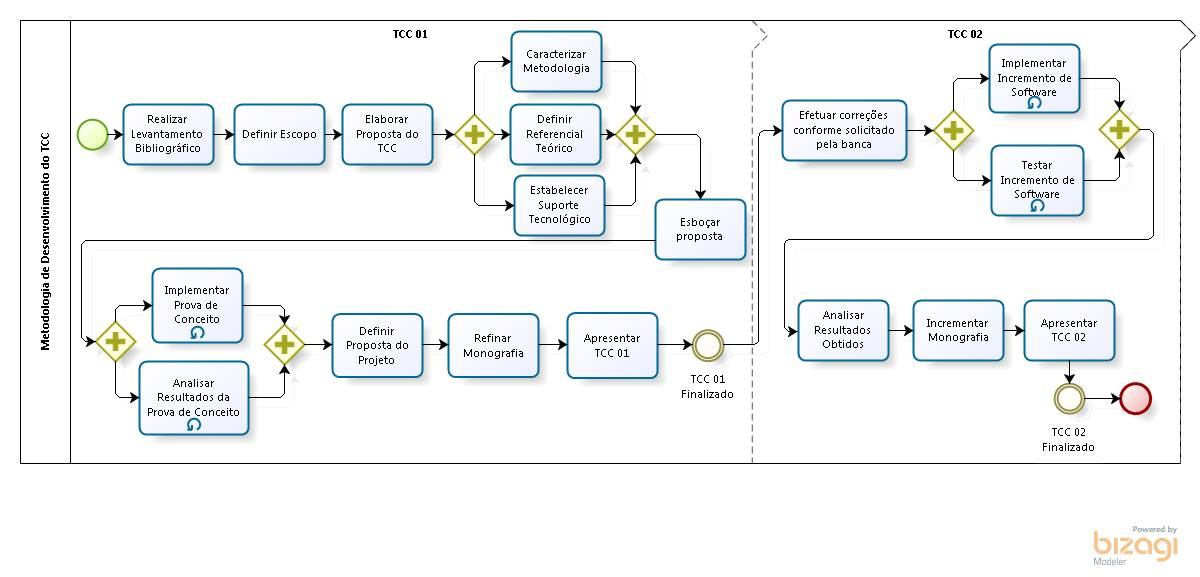
\includegraphics[width=\textwidth]{figuras/processo.jpg}
    \caption{Fluxo de atividades do trabalho de conclusão de curso}
    \label{fig:processo}
  \end{figure}

\par 
\indent A Figura \ref{fig:processo} representa o fluxo de atividades utilizado no trabalho de conclusão de curso, como descrito anteriormente.  
  
    \begin{figure}[h]
    \centering
    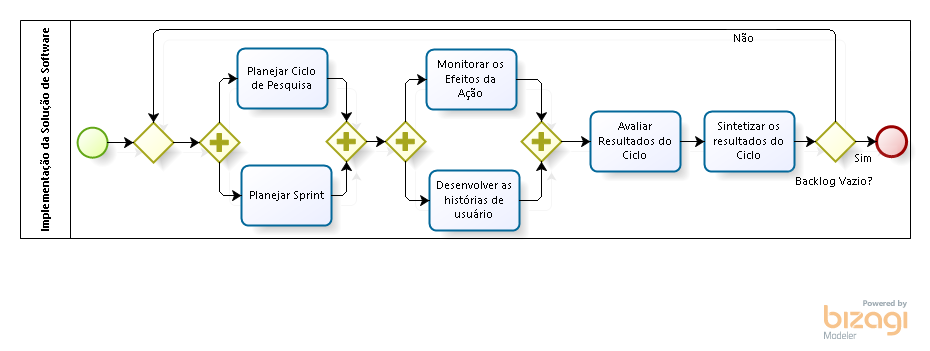
\includegraphics[width=\textwidth]{figuras/ProcessoInterno.png}
    \caption{Fluxo de atividades da implementação da solução de software}
    \label{fig:processointerno}
  \end{figure}

\par 
\indent A Figura \ref{fig:processointerno} demonstra a adaptação do Scrum e o uso de pesquisa-ação no desenvolvimento do \textit{framework}. 
 
\subsection{Detalhes da Execução do Desenvolvimento}
	Inicialmente, definiu-se os requisitos iniciais do projeto. Para esse fim, foi especificado um épico que atende o objetivo geral do projeto: \textsf{Geração de Testes Unitários a partir de marcações em comentários no próprio código fonte}. A partir desse épico, foram derivados as seguintes \textit{features}:
	\begin{description}
	\item[Identificação dos elementos da linguagem de programação Grails:] permitir que o gerador de testes seja capaz de identificar os elementos da linguagem de programação Grails, garantindo análises futuras;
	\item[Análise dos métodos da camada de domínio (\textit{model}):] permitir que o gerador faça uma análise dos métodos presentes nas classes de domínio, produzindo casos de teste específicos para cada método desta camada;
	\item[Análise dos métodos da Camada de Controle (\textit{controller}):] permitir que o gerador faça uma análise dos métodos presentes nas classes controladoras, produzindo casos de teste específicos para cada método desta camada;
	\item[Desenvolvimento do Framework:] permitir que o gerador criado possa ser extensível e adaptável para diferentes linguagens de programação.
	\end{description}
\par
\indent O detalhamento de cada \textit{feature} ocorreu conforme execução do projeto e maior entendimento do desenvolvimento de cada funcionalidade.

\subsubsection{FE01 Identificação dos elementos da linguagem de programação Grails}
Esse funcionalidade é responsável pela criação da gramática capaz de identificar a linguagem de programação Grails. Para isso, foram identificadas 10 histórias de usuários que estão listadas na Tabela \ref{feature01}. Essa \textit{feature} foi a primeira detalhada e implementada. No desenvolvimento, houve dificuldade de construir uma gramática com o mínimo de conflitos possível, capaz de identificar toda a linguagem Grails e, por esse motivo, a implementação dessa funcionalidade foi concluída na \textit{sprint} 3.

\subsubsection{FE 02 Análise dos métodos da camada de domínio (\textit{model})}
Essa funcionalidade engloba a análise e a criação dos testes de modelo. Embora a quantidade de histórias de usuários desse \textit{feature} seja reduzida, a dificuldade técnica associada foi desafiadora. Objetivou-se, nesse momento, concluir um gerador de testes para \textit{model} que fosse capaz de gerar casos de testes para métodos da camada de modelo. Esse funcionalidade foi implementada nas \textit{sprints} 4 e 5 e as histórias relacionadas estão listadas na Tabela \ref{feature02}.

\subsubsection{FE 03 Análise dos métodos da Camada de Controle (\textit{controller})}
Funcionalidade similar à \textit{feature} 02, cujo objetivo pode ser resumido na geração de testes. Entretanto, a \textit{feature} 03 focou em gerar testes para a camada de controle. Os métodos abordados foram os responsáveis pela criação, leitura, atualização e exclusão de uma classe. A implementação dessa funcionalidade ocorreu em paralelo com a \textit{feature} 02, ou seja, nas \textit{sprints} 4 e 5. Segue, na Tabela \ref{feature03}, as histórias dessa funcionalidade.

\subsubsection{FE 04 Desenvolvimento do Framework}
A \textit{feature} 04 visou tornar o gerador de testes em um \textit{framework}, tornando-o extensível e adaptável para diferentes linguagens de programação. Para isso, foi necessário identificar os pontos do software que são genéricos para qualquer linguagem e os pontos que são adaptáveis, conhecidos como \textit{hotspots}. Para auxiliar nesse processo, utilizou-se diagramas de classe e de sequência. Em seguida, executou-se uma refatoração aplicando os padrões de projeto identificados como candidatos e, por fim, documentou-se o uso do \textit{framework}. Essa funcionalidade foi implementada na \textit{sprint} 6, e suas histórias estão detalhadas na Tabela \ref{feature04}.

\begin{table}[h]
\centering
\caption{Histórias da \textit{feature} 01}
\label{feature01}
\begin{tabular}{@{}cccc@{}}
\toprule
 
\textbf{ID} & \textbf{Descrição} & \textbf{Pt.} & \textbf{Status} \\ \toprule
US01 & \begin{tabular}[c]{@{}c@{}}Eu, como desenvolvedor, quero identificar os elementos\\ da declaração de variáveis, para análises futuras desses elementos.\end{tabular} & 3 & Feito \\ \hline
US02 & \begin{tabular}[c]{@{}c@{}}Eu, como desenvolvedor, quero identificar os elementos\\ de declarações iniciais, para análises futuras desses elementos.\end{tabular} & 3 & Feito \\ \hline
US03 & \begin{tabular}[c]{@{}c@{}}Eu, como desenvolvedor, quero identificar os elementos\\ de atribuição de variáveis, para análises futuras desses elementos.\end{tabular} & 3 & Feito \\ \hline
US04 & \begin{tabular}[c]{@{}c@{}}Eu, como desenvolvedor, quero identificar os elementos \\ de declaração de classes, para análises futuras desses elementos.\end{tabular} & 3 & Feito \\ \hline
US05 & \begin{tabular}[c]{@{}c@{}}Eu, como desenvolvedor, quero identificar os elementos\\ de declaração de métodos, para análises futuras desses elementos.\end{tabular} & 3 & Feito \\ \hline
US06 & \begin{tabular}[c]{@{}c@{}}Eu, como desenvolvedor, quero identificar os elementos\\ de declaração de estruturas condicionais, para análises\\  futuras desses elementos.\end{tabular} & 3 & Feito \\ \hline
US07 & \begin{tabular}[c]{@{}c@{}}Eu, como desenvolvedor, quero identificar os elementos\\ de declaração estruturas de repetição, para análises \\ futuras desses elementos.\end{tabular} & 3 & Feito \\ \hline
US08 & \begin{tabular}[c]{@{}c@{}}Eu, como desenvolvedor, quero identificar os elementos\\ de comentários, para análises futuras desses elementos.\end{tabular} & 3 & Feito \\ \hline
US09 & \begin{tabular}[c]{@{}c@{}}Eu, como desenvolvedor, quero identificar elementos\\ de expressões da linguagem grails, \\ para análises futuras desses elementos.\end{tabular} & 5 & Feito \\ \hline
US10 & \begin{tabular}[c]{@{}c@{}}Eu, como desenvolvedor, quero identificar elementos\\ que forma uma strings, para análises futuras desses elementos.\end{tabular} & 3 & Feito \\ \hline
\end{tabular}
\end{table}

\begin{table}[h]
\centering
\caption{Histórias da \textit{feature} 02}
\label{feature02}
\begin{tabular}{@{}cccc@{}}
\toprule
\textbf{ID} & \textbf{Descrição} & \textbf{Pt.} & \textbf{Status} \\ \toprule
US11 & \begin{tabular}[c]{@{}c@{}}Eu, como desenvolvedor, quero analisar métodos\\  de validação de classes de domínio, para gerar casos de testes.\end{tabular} & 8 & Feito \\ \hline
US12 & \begin{tabular}[c]{@{}c@{}}Eu, como desenvolvedor, quero analisar métodos \\ de instanciação de classes de domínio, para gerar casos de testes.\end{tabular} & 8 & Feito \\ \hline
US13 & \begin{tabular}[c]{@{}c@{}}Eu, como desenvolvedor, quero analisar métodos \\ de relacionamento de classes de domínio, para gerar casos de testes\end{tabular} & 8 & Feito \\ \hline
\end{tabular}
\end{table}

\begin{table}[h]
\centering
\caption{Histórias da \textit{feature} 03}
\label{feature03}
\begin{tabular}{@{}cccc@{}}
\toprule
\textbf{ID} & \textbf{Descrição} & \textbf{Pt.} & \textbf{Status} \\ \toprule
US14 & \begin{tabular}[c]{@{}c@{}}Eu, como desenvolvedor, quero analisar métodos de\\ criação de classes controladoras, para gerar casos de testes.\end{tabular} & 8 & Feito \\ \hline
US15 & \begin{tabular}[c]{@{}c@{}}Eu, como desenvolvedor, quero analisar métodos de\\ exclusão de classes controladoras, para gerar casos de testes.\end{tabular} & 8 & Feito \\ \hline
US16 & \begin{tabular}[c]{@{}c@{}}Eu, como desenvolvedor, quero analisar métodos de\\ alteração de classes controladoras, para gerar casos de testes.\end{tabular} & 8 & Feito \\ \hline
US17 & \begin{tabular}[c]{@{}l@{}}Eu, como desenvolvedor, quero analisar métodos de\\ visualização de classes controladoras, para gerar casos de testes.\end{tabular} & 8 & Feito \\ \hline
\end{tabular}
\end{table} 

\begin{table}[h]
\centering
\caption{Histórias da \textit{feature} 04}
\label{feature04}
\begin{tabular}{@{}cccc@{}}
\toprule
\textbf{ID} & \textbf{Descrição} & \textbf{Pt.} & \textbf{Status} \\ \toprule
US18 & \begin{tabular}[c]{@{}c@{}}Eu, como desenvolvedor, quero identificar os pontos de\\ generalização e hotspots, para criação do framework.\end{tabular} & 5 & Feito \\ \hline
US19 & \begin{tabular}[c]{@{}c@{}}Eu, como desenvolvedor, quero implementar padrão de projeto Builder,\\ para facilitar a criação de arquivos de testes em outras linguagens.\end{tabular} & 8 & Feito \\ \hline
US20 & \begin{tabular}[c]{@{}c@{}}Eu, como desenvolvedor, quero implementar padrão de projeto Factory,\\ para facilitar a criação de arquivos de coleta de dados em outras linguagens.\end{tabular} & 8 & Feito \\ \hline
US21 & \begin{tabular}[c]{@{}c@{}}Eu, como desenvolvedor, quero refatorar o framework desenvolvido,\\ para facilitar na adaptação e uso em outras linguagens.\end{tabular} & 5 & Feito \\ \hline
US22 & \begin{tabular}[c]{@{}c@{}}Eu, como desenvolvedor, quero documentar o framework,\\ para facilitar o seu uso.\end{tabular} & 5 & Feito \\ \hline
\end{tabular}
\end{table}
 
 \subsection{Cronograma}
 Os cronogramas a seguir evidenciam a execução, visão temporal, das atividades referentes ao trabalho de conclusão de curso como um todo, incluindo as atividades referentes ao TCC\_01 e ao TCC\_2.
	  
\begin{table}[h]
  \tiny
  \centering
  \caption{Cronograma para o trabalho de conclusão de curso 1}
  \label{cronograma-tcc-1}
  \begin{tabular}{@{}cccccc@{}}
    \toprule
    Atividades & Agosto & Setembro & Outubro & Novembro & Dezembro \\ \toprule
    Realizar Levantamento Bibliográfico & X &  &  &  &  \\
    Definir Escopo & X &  &  &  &  \\
    Elaborar Proposta Inicial do TCC & X & X &  &  &  \\
    Caracterizar Metodologia &  & X &  &  &  \\
    Definir Referencial Teórico &  & X &  &  &  \\
    Estabelecer Suporte Tecnológico &  & X &  &  &  \\
    Esboçar Proposta &  & X & X &  &  \\
    Implementar Prova de Conceito &  &  & X &  &  \\
    Analisar Resultados da Prova de Conceito &  &  & X &  &  \\
    Definir Proposta do Projeto &  &  &  & X &  \\
    Refinar Monografia &  &  &  & X &  \\
    Apresentar TCC 01 &  &  &  & X & X \\ \hline
  \end{tabular}
\end{table}
\FloatBarrier
  
\begin{table}[h]
  \tiny
  \centering
  \caption{Cronograma para o trabalho de conclusão de curso 2}
  \label{cronograma-tcc-2}
  \begin{tabular}{@{}cccccc@{}}
  \toprule
    Atividades & Fevereiro & Março & Abril & Maio & Junho \\ \toprule
    Efetuar Correções conforme solicitado pela banca & X &  &  &  &  \\
    Implementar Incremento de Software &  & X & X & X &  \\
    Testar Incremento de Software &  & X & X & X & X \\
    Analisar Resultados Obtidos &  &  & X & X & X \\
    Incrementar Monografia &  &  &  &  & X \\
    Apresentar TCC 2 &  &  &  &  & X \\ \hline
  \end{tabular}
\end{table}
\FloatBarrier
  
  \section{Resumo do Capítulo}
  Este capítulo abordou sobre as metodologias de pesquisa, classicando-as em dois aspectos: quanto ao objetivo e aos procedimentos técnicos. Foi definida uma adaptação da metodologia de pesquisa-ação e Scrum. Em seguida, detalhou-se o fluxo de atividades do projeto, e apresentou-se a execução das atividades no cronograma.